% !TEX root = /Users/zhuzhuangdi/Desktop/MSUCourses/NaturalLanguageProcessing842/CSE842/FinalReport/latex/final.tex

\section{DeepTweeting Sentiment Analysis System} 
We implement a system that utilizes a recursive a Recurrent Neural Network (RNN) model to predict the sentiment classes of different tweets.
%
Especially, we use a specialized RNN named Long Short Term Memory (LSTM) network as our system model.
%
We adopt two pre-processing steps to map each tweet into a three-dimensional matrix representation, so that the relevant meaning among different words in the Twitter corpus can be captured.
%
The output of our model is a probability distribution of all the sentiment labels for a tweet.
%
In our project, we only consider two-class sentiment classifications, that is, a tweet can be either negative or positive.
%
However, our model can be easily scaled to multi-sentiment classification problems. Our system overview is shown in Figure \ref{fig:systemoverview}.

\begin{figure}[htb]
	\centering
	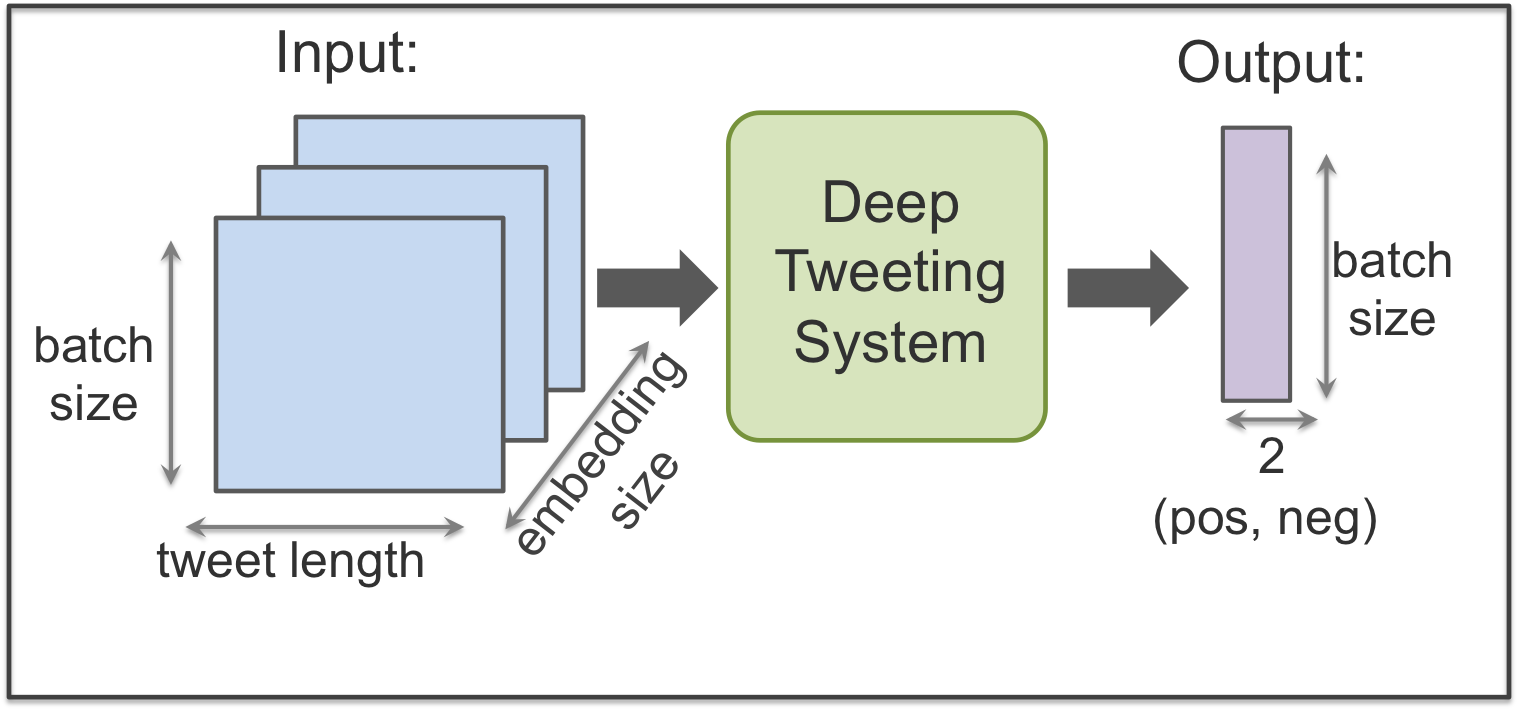
\includegraphics[width=0.9\linewidth]{DeepTweetingOverview}
	\caption{Sentiment Analysis System Overview}
	\label{fig:systemoverview}
\end{figure}


% based on the vector-space representation of the tweet.
%The intuition is that: for sentence-level messages like tweets, the meaning of this expression should be derived based on the meanings of its words and the rules used to combine them.
%We will semantic compositionnality of tweets, and generate a parse tree for each tweet as the input of this model.  
%
%the Stanford Parser\cite{klein2003accurate} to for parse tree generation.
%

%proposed by \cite{kouloumpis2011twitter} %
%Moreover, we  also plan to explore the possibility to use hashtags and emotions as feature to improve the sentiment classification accuracy of our model.
%
%of pairs of words whereas we would like nonlinear functions to compute compositional meaning representations for multi-word phrases or full sentences.
%
%For evaluation, we plan to use two baselines to compare with our approach: a Naive-Bayesian model using bi-grams as features, and an SVM model using Term frequency ITF-IDF as features.
%
%%As a special task for sentence-level sentiment analysis, twitter sentiment analysis 
%The features of informal language, the frequent use of emotions and hashtags, as well as the lengths constraints of tweets make the analysis of twitter 




%It's an open question how well the features and techniques used on more well-formed data will transfer to the microblogging domain.
%Many researchers, such as Mullen and Collier \cite{mullen2004sentiment}, have used empirical distributions of words and hand-selected features to perform this analysis with a variety of standard machine learning models, such as SVMs and Naive-Bayes.
%These approaches have been effective on certain datasets, but have poor cross-domain performance and require significant domain-specific tailoring. 
%
%These prove to be a weak point in many models. 
%Therefore, we can take from this that explicit modeling of these more complicated linguistic effects can be beneficial to any sort of semantic analysis - in particular, including sentiment analysis. 
%%
%%Additionally, the datasets these models are based upon generally only contain sentiment labels for the entire sentence, making it ambiguous which part of the sentence was responsible for the sentiment.
%The very nature of the microblogging domain make Twitter sentiment analysis a very special task in sentence-level sentiment classification task.
 
\subsection{Preprocessing}
We use word embedding to map Chinese characters from the poem corpus to vectors of real numbers, which consists of two steps: tokenization and word embedding.
% 
%Especially, we consider both semantic and rhythmic relevance in the word-to-vector transformation.
%
\subsubsection {Tweet Tokenization}
%We associated each Chinese character with a unique value as its ID, so that the most frequent word in the corpus  will get a highest value, while the less frequent words have smaller ones.
%During our project, we carefully tune the size of the vocabulary set $|V|$ so that the most $|V|$ frequent words will be kept in our vocabulary, while the other unfrequent words will be mapped to the same \emph{UNKOWN} token to avoid overfitting.
%
Then we use the ID as the feature for each word to train our word embedding matrix.
%Each character has a unique index ID, while characters share the same simple or compound vowels will have the same rhyme ID. 
%For example, in Figure \ref{fig:rhyme_features}, the two Chinese characters, \emph{guang} and \emph{shuang}, will maintain the same rhyme ID.
%The rhymes can be extracted using a python module called \emph{pinyin}.
%
As a specialized corpus, tweet data contain large amount of micro-blogging features, such as emojis, hand-shorts, hashtags and user mentions \cite{kouloumpis2011twitter}.
%
A straight-forward approach to preprocess these data is to consider all above features as noises and remove them from each tweet.
%
However, this may lead to information loss, as this micro-blogging features usually reveal strong sentiment trends.
%
So our approach is to map each kind of above-mentioned feature into a specific keyword using regular expression:
\begin{itemize}
\item Emotions: We map all different kinds of emotions in a tweet to the same keyword ${<emoji>}$.
\item Shorthands: We collect most popular shorthands in twitter. For each tweet, we convert the shorthands in it into a phrase revealing its sentimental tendency. For example, \emph{3$>$} means \emph{love}.
\item Hashtags: We seperate the hashtag from its following word, and map the hashtag to a keyword \emph{hashtag}. For example, $\# amazing$ will be $<hashtag>$ $amazing$.
\item Mentions: we map all user mentions to a keyword ${<user>}$. 
\item Duplications: For each word in a tweet, if there are duplicate letters for more than three times, such as \emph{cooooooool}, we will only keep two letters of them, so the above-mentioned word will change to \emph{cool}.
\item URLs: Since URLs are usually irrelevant with the sentiment tendency of the tweet, so we just replace all URLs in tweets with a keyword $<URL>$.
\end{itemize} 


\begin{figure}[ht]
% \hspace{-0.2in}
\begin{minipage}[t]{1\linewidth}
\centering 
\subfigure[]{
   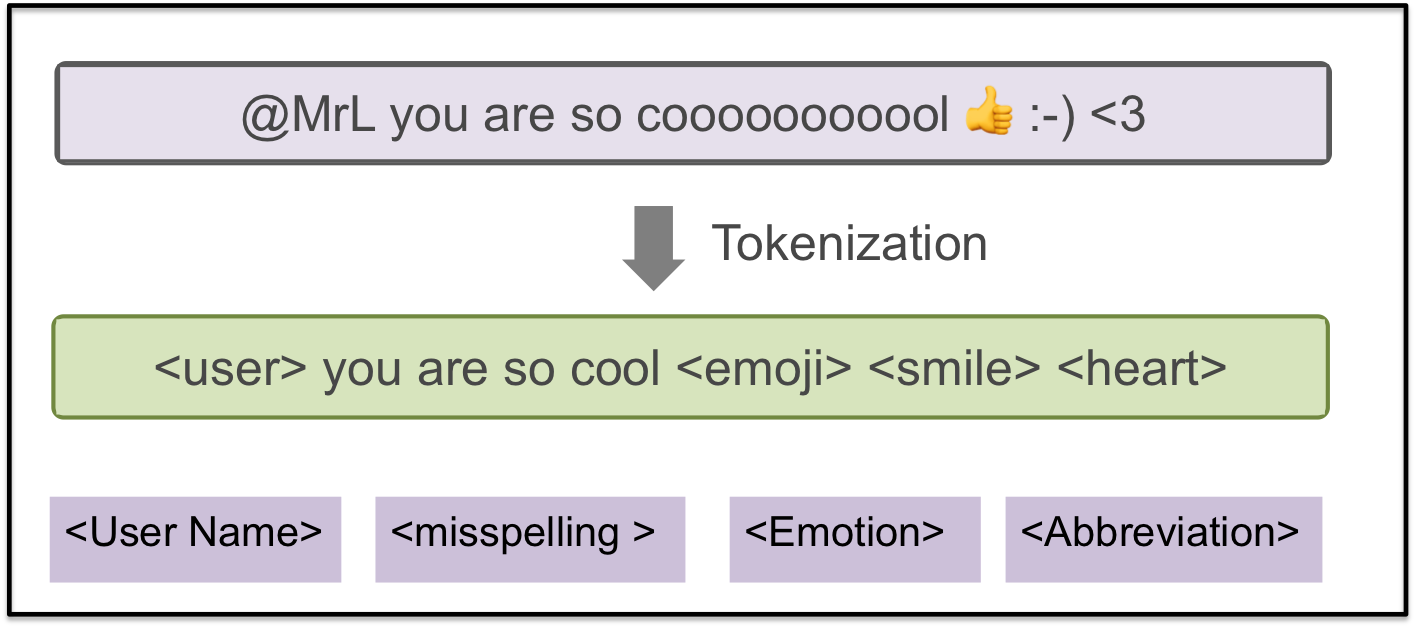
\includegraphics[width=0.9\linewidth] {token1}
   \label{fig:token1}
 } 
% \hspace{-0.2in}
 \subfigure[]{
   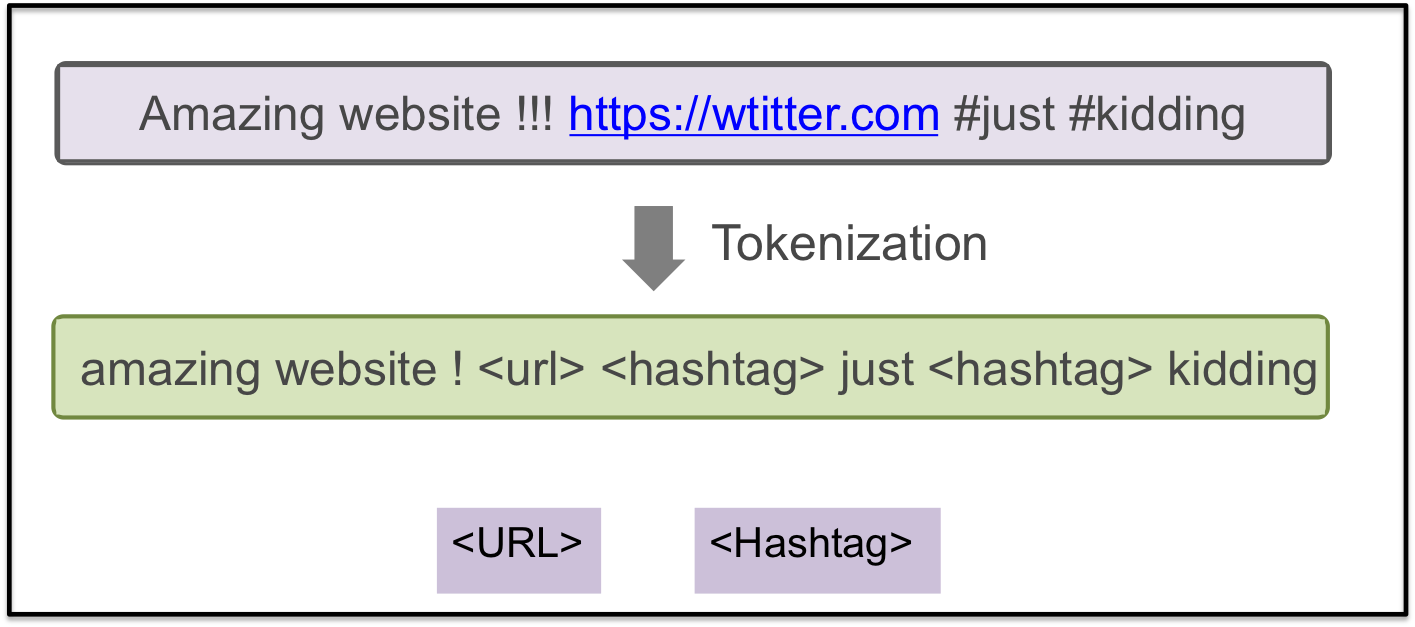
\includegraphics[width=0.9\linewidth] {token2}
   \label{fig:token2}
 } 
\caption{\textbf{Twitter Tokenization with respect to different micro-blogging features}}
\label{fig:token}
\end{minipage}
\end{figure}


\subsubsection {Word to Vector Representation}
We cannot feed our RNN model with raw tweet text, so a vector representation for tweet is necessary.
%
Especially, we adopt a skip-gram model to get a word-embedding matrix for all words in the Twitter corpus\cite{mikolov2013efficient}, so that the semantic relevance  among different words can be captured and used as inputs to the RNN model.
%
We get this matrix by training a single-layer neural network. 
%and the parameter matrix inside the network will be our word embedding matrix.
%
 The input of the model is a single word $w_I$, and the output is the words in its context $\{w_{O,1},w_{O,2}, \dots, w_{O,C}\}$ defined by a word window of size $C$.
%
As shown in Figure \ref{fig:skip_gram},  $x$ represents the one-hot encoded vector corresponding to the
input word in the training text,
%
 and $\{y_1, y_2, \dots, y_C\}$ are the one-hot encoded vectors corresponding to the output words in the training text.
 %
 The $V \times N$ matrix $W$ is the weight matrix between the input layer and hidden layer whose
$i^{th}$ row represents the weights corresponding to the $i^{th}$ word in the vocabulary. 
%
This weight matrix is what we call the word-embedding matrix because it contains the
vector encodings of all of the words in our vocabulary.
%
We can use this word-embedding matrix to capture the semantic relevance among words, so that two words with close semantic meanings will have smaller distance in the vector space.

\begin{figure}[htb]
	\centering
	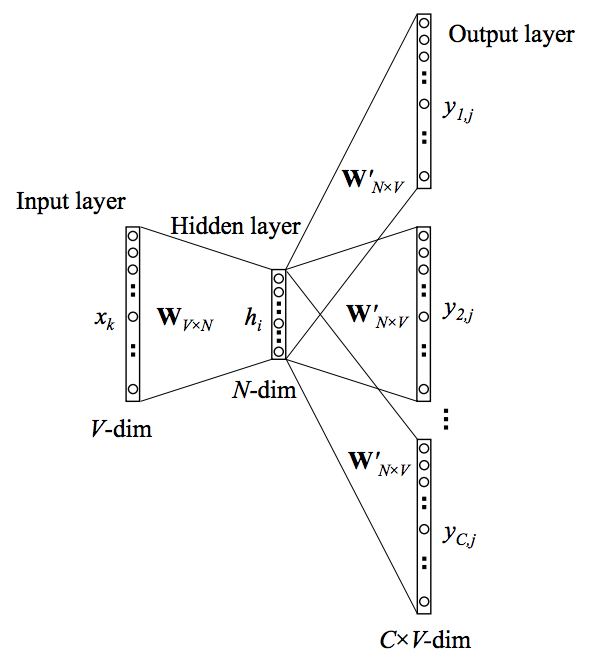
\includegraphics[width=0.9\linewidth]{skip_gram}
	\caption{A skip gram neural network}
	\label{fig:skip_gram}
\end{figure} 

\begin{figure}[htb]
	\centering
	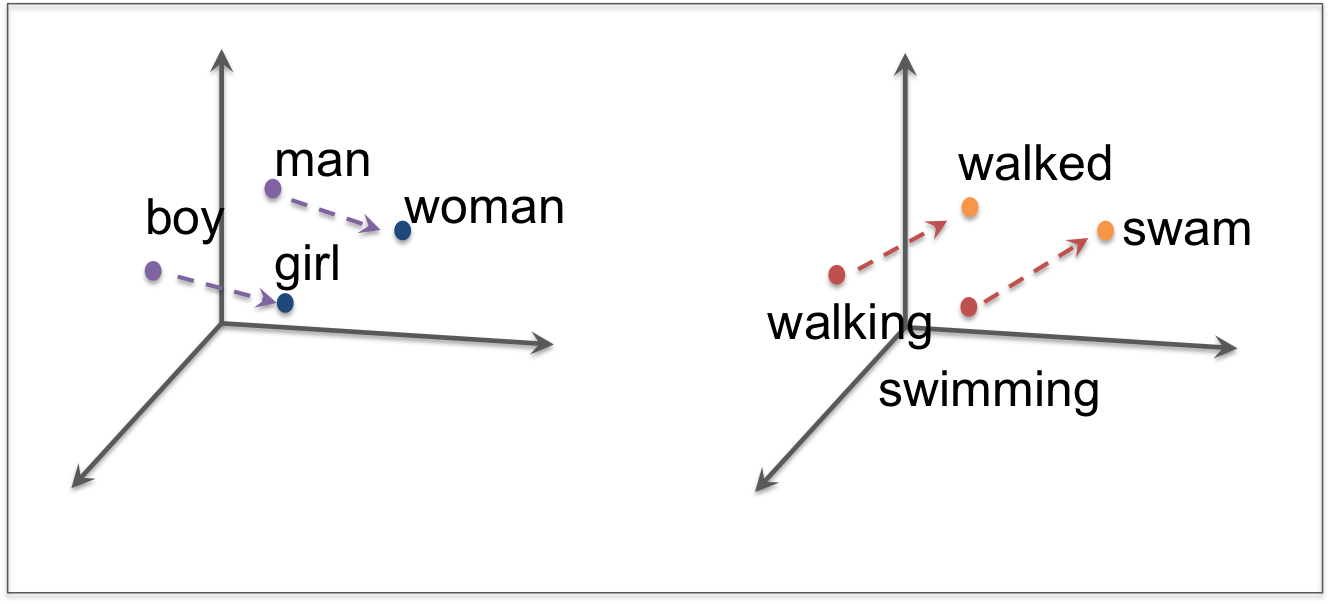
\includegraphics[width=0.9\linewidth]{word2vec}
	\caption{Vector Representation of words}
	\label{fig:word2vec}
\end{figure}


\subsection{Recurrent Neural Network}  
Recurrent Neural Networks (RNN)s are a specialized neural network that consists of multiple copies of the same network cell, as shown in Figure \ref{rnn_overview}.
%
Due to this recursive structure, it is suitable for processing sequential data  \cite{rumelhart1986}.
%
%It is specialized for processing a sequence of valuesx $x^{(1)}, x^{(2)}, \dots, x^{(t)}$.
%
For each network cell $A_t$ in the RNN model, its has an input $s_t$, a hidden state $s_t$, and generates an output $h_t$.
%
The output and hidden state are then scaled and feed as inputs to its successor network cell.
%Parameter sharing across the different parts of the model is the key idea that makes RNNs to be able to deal with the sequential data.
%
However, a simple RNNs cannot learn long time dependency, because during the optimization step, the parameter matrix this term tends to vanish or explode very fast due stochastic gradient \cite{goodfellow2016deeplearning}.
%
To solve this challenge, specialized RNNs with gates is proposed and becomes one of the most effective practical models that used for sequential data.
\begin{figure}[htbp]
	\centering
	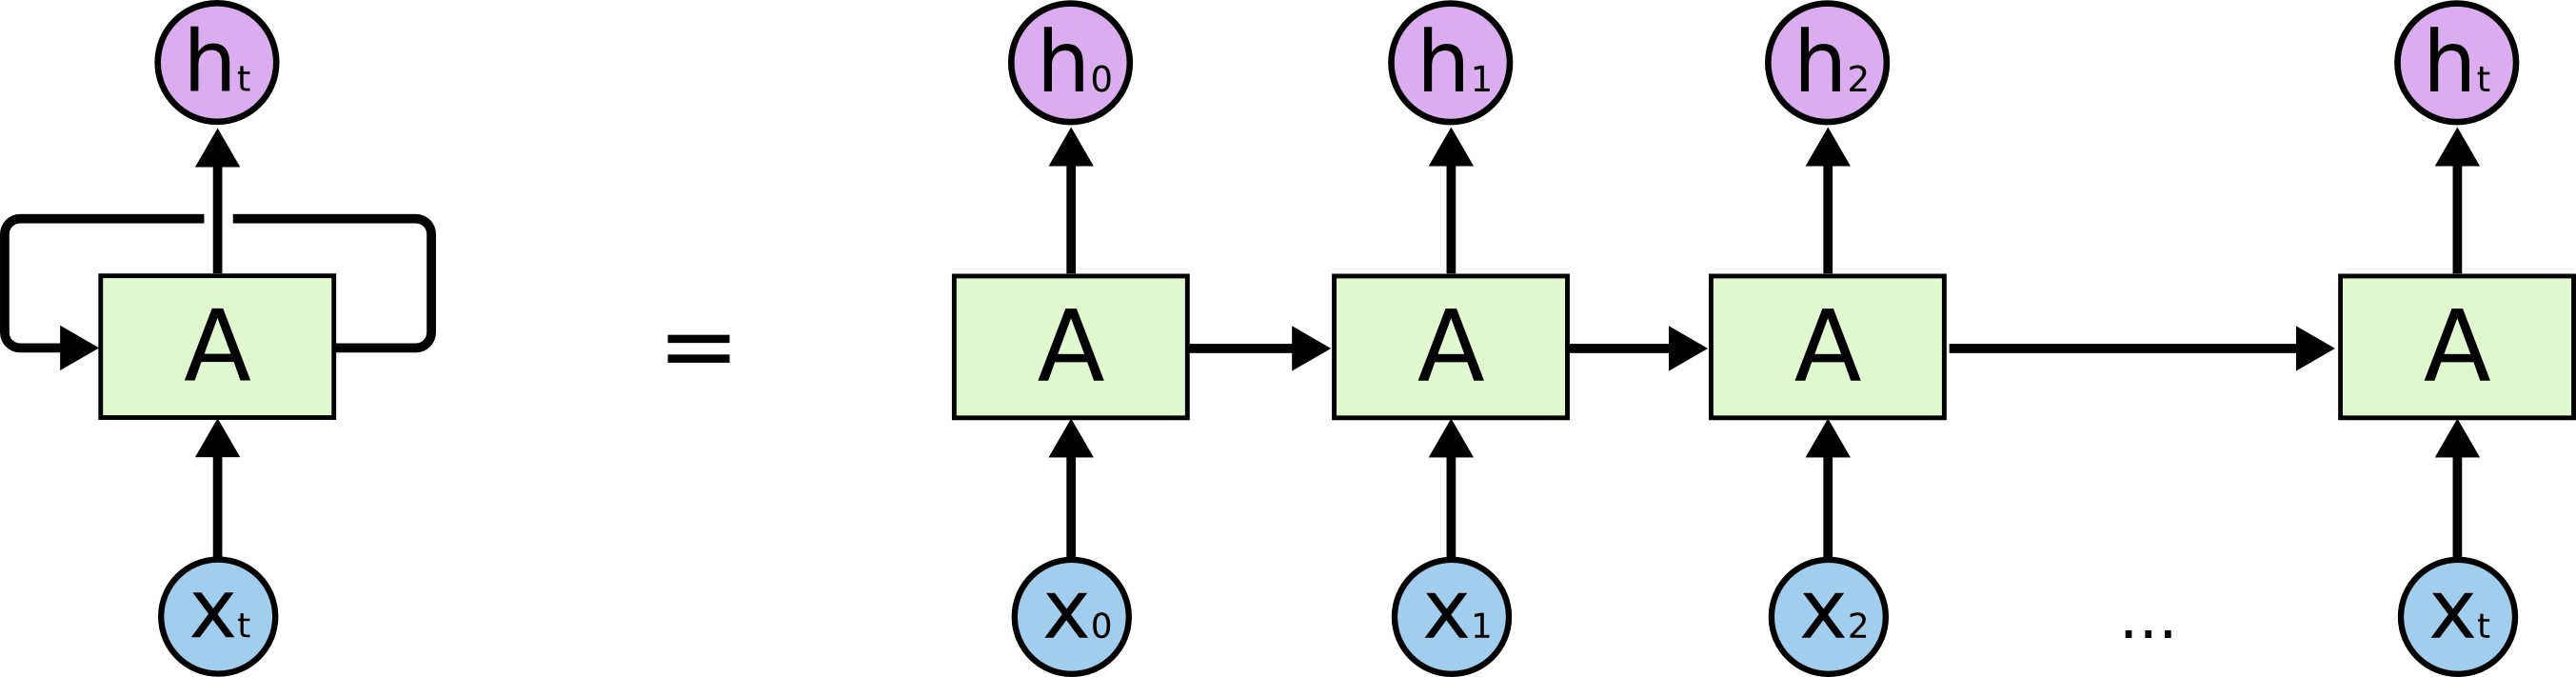
\includegraphics[width=0.9\linewidth]{rnn_overview}
	\caption{A Recurrent Neural Network}
	\label{fig:rnn_overview}
\end{figure}




\subsubsection{Long Short Term Memory}
In our project, we will use a specialized RNN network called Long Short Term Memory (LSTM).
%
Long Short Term memory (LSTM) network is a branch of gated RNNs that can capture long term dependencies when processing sequences of input texts..
%
It is widely used in various machine learning and NLP applications, such as speech recognition, machine translation, and handwriting generation\cite{hochreiter1997lstm} .
%
Gates are a way to optionally let information through. They are composed out of a sigmoid neural net layer and a pointwise multiplication operation. 
%
A LSTM network contains recursive LSTM network cells, each of which consists of the following gates:
\begin {itemize}
\item {Forget gate \(f_i\):} 
\[ f_t =  \sigma (W_f \dot [h_{t-1} , x_t] + b_f ) \]
%\[f_i^{(t)} = \sigma (b_i^f + \sum_{j}U_{i,j}^f x_j^{(t)} +\sum_{j}W_{i,j}^f h_j^{(t-1)} ) \].
%
It generates a scale parameter between 0 and 1 for each component in the previous LSTM cell $C_{t-1}$, based on the current input $x_t$ and previous output \( h_{t-1} \).
%
%Where \(\boldsymbol{x}^{(t)}\) is the current input vector and \(\boldsymbol{h}^{(t)}\) is the current hidden layer vector, containing the outputs of all the LSTM cells. \(\boldsymbol{b}^f\), \(\boldsymbol{U}^f\), and \(\boldsymbol{W}^f\) are biases, input weights, and recurrent weights of the forget gate, respectively. 

\item {External input gate \(i_t \): } the external input gate unit is computed with the following equation:
\[i_t = \sigma (b_i +  W_i  \dot [h_{t-1}, x_t] ) \]

\item {Update gate \( \tilde{C_t} \):} 
This gate updates the internal state of the LSTM cell by the following equation:
\begin{small}
\[  \tilde{C_t} = \tanh (W_C \dot [h_{t-1}, x_t ] + b_C )  \]
\end{small}

\item {Output gate \(h^{(t)}\) and \(q_i^{(t)}\) :}  The output \(h^{(t)}\)
and the output gate \(q_i^{(t)}\) are updated using sigmoid function also:
\begin{eqnarray*}
o_{(t)} &=& \sigma (W_o [h_{t-1} , x_t ] + b_o ) \\
h{(t)} &=& \tanh (C_t) o_{(t)}
\end{eqnarray*}

\end{itemize}



%The key idea of LSTM is to introduce a self loop so that . 
%As shown in Figure \ref{fig:lstm}, the self loop (internal recurrence) is located in "LSTM cells" with outer recurrence like ordinary recurrent network. The weight of self-loop is controlled by a forget gate 
 
  

Using the above four gates in a LSTM cell,  the gradient can flow for long duration , and therefore LSTM can learn long-term dependencies more effectively than normal RNNs. 

\begin{figure}[htb]
	\centering
	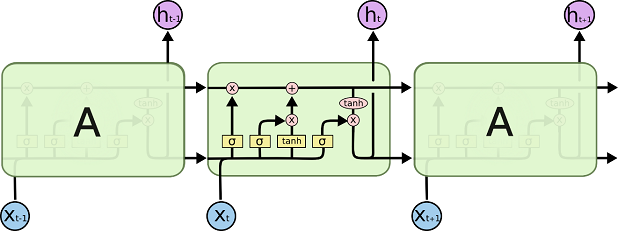
\includegraphics[width=0.9\linewidth]{lstm}
	\caption{A Long Short Term Memory network}
	\label{fig:lstm}
\end{figure} 

\begin{figure}[ht]
% \hspace{-0.2in}
\begin{minipage}[t]{1\linewidth}
\centering 
\subfigure[RNN]{
   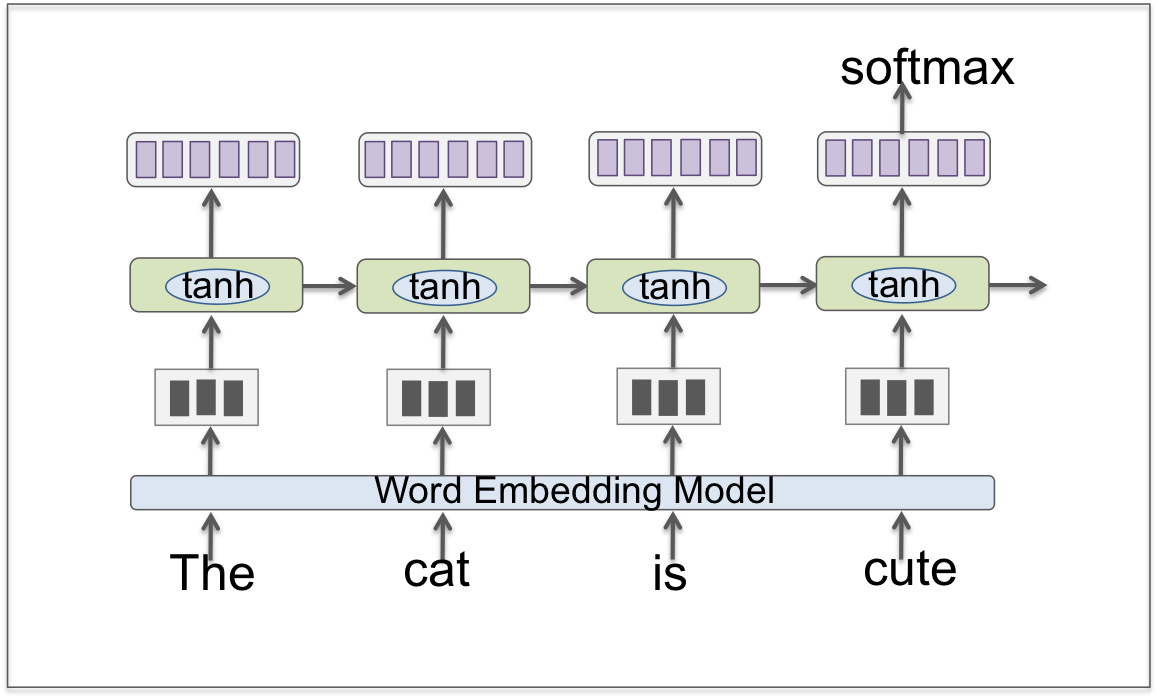
\includegraphics[width=0.9\linewidth] {rnn_workflow}
   \label{fig:rnn_workflow}
 } 
% \hspace{-0.2in}
 \subfigure[LSTM]{
   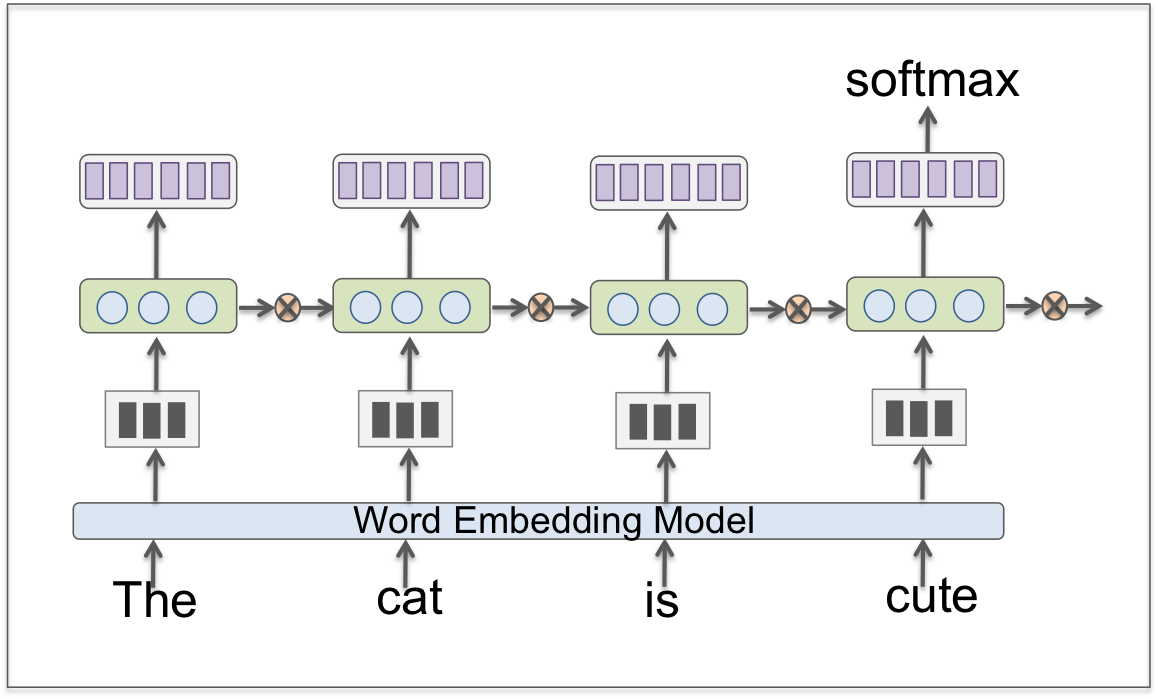
\includegraphics[width=0.9\linewidth] {lstm_workflow}
   \label{fig:lstm_workflow}
 } 
\caption{\textbf{RNN model and LSTM model for sentiment analysis}}
\label{fig:songci}
\end{minipage}
\end{figure}



